\documentclass{article}%
\usepackage{amsmath}%
\usepackage{amsfonts}%
\usepackage{amssymb}%
\usepackage{graphicx}
\usepackage{enumitem}
\usepackage{tikz,pgfplots}
%-------------------------------------------
\newtheorem{theorem}{Theorem}
\newtheorem{acknowledgement}[theorem]{Acknowledgement}
\newtheorem{algorithm}[theorem]{Algorithm}
\newtheorem{axiom}[theorem]{Axiom}
\newtheorem{case}[theorem]{Case}
\newtheorem{claim}[theorem]{Claim}
\newtheorem{conclusion}[theorem]{Conclusion}
\newtheorem{condition}[theorem]{Condition}
\newtheorem{conjecture}[theorem]{Conjecture}
\newtheorem{corollary}[theorem]{Corollary}
\newtheorem{criterion}[theorem]{Criterion}
\newtheorem{definition}[theorem]{Definition}
\newtheorem{example}[theorem]{Example}
\newtheorem{exercise}[theorem]{Exercise}
\newtheorem{lemma}[theorem]{Lemma}
\newtheorem{notation}[theorem]{Notation}
\newtheorem{problem}[theorem]{Problem}
\newtheorem{proposition}[theorem]{Proposition}
\newtheorem{remark}[theorem]{Remark}
\newtheorem{solution}[theorem]{Solution}
\newtheorem{summary}[theorem]{Summary}
\newcommand\abs[1]{\left|#1\right|}
\newcommand\EXP[1]{\exp\left(#1\right)}
\newenvironment{proof}[1][]{\begin{samepage}\textbf{Proof #1} \\ }{\\ \rule{0.5em}{0.5em} \end{samepage} \\}
\setlength{\textwidth}{7.0in}
\setlength{\oddsidemargin}{-0.35in}
\setlength{\topmargin}{-0.5in}
\setlength{\textheight}{9.0in}
\setlength{\parindent}{0.3in}
\begin{document}

\begin{flushright}
\textbf{Brandon Toner \\
\today}
\end{flushright}

\begin{center}
\textbf{MATH 438: Introduction to Complex Variables \\
Assignment 2} \\
\end{center}

\begin{enumerate}
    \item %1
    \begin{enumerate}[label=\alph*]
    
\item \leavevmode\vadjust{\vspace{-\baselineskip}}\newline %a

            \begin{tikzpicture}
                \draw (0,0) -- coordinate (x axis mid) (5,0);
                \draw (0,0) -- coordinate (y axis mid) (0,5);
                %ticks
                    \foreach \x in {0,...,5}
                        \draw (\x,1pt) -- (\x,-3pt)
                            node[anchor=north] {\x};
                    \foreach \y in {0,...,5}
                        \draw (1pt,\y) -- (-3pt,\y) 
                            node[anchor=east] {\y}; 
                \draw(1,1) circle (1);
            \end{tikzpicture}

\item \leavevmode\vadjust{\vspace{-\baselineskip}}\newline

                    \begin{tikzpicture}

            \draw[fill=black!50] (3,0) circle (1);
            \draw[fill=white] (3,0) circle (0.5);


            \draw (0,0) -- coordinate (x axis mid) (5,0);
            \draw (0,0) -- coordinate (y axis mid) (0,5);
             %ticks
                 \foreach \x in {0,...,5}
                     \draw (\x,1pt) -- (\x,-3pt)
                         node[anchor=north] {\x};
                 \foreach \y in {0,...,5}
                     \draw (1pt,\y) -- (-3pt,\y)
                         node[anchor=east] {\y};
             \end{tikzpicture}

\item \leavevmode\vadjust{\vspace{-\baselineskip}}\newline %c
                    \begin{tikzpicture}
            \draw[fill=black!40] (3,0) circle (1.732);

            \draw (0,0) -- coordinate (x axis mid) (5,0);
            \draw (0,0) -- coordinate (y axis mid) (0,5);
             %ticks
                 \foreach \x in {0,...,5}
                     \draw (\x,1pt) -- (\x,-3pt)
                         node[anchor=north] {\x};
                 \foreach \y in {0,...,5}
                     \draw (1pt,\y) -- (-3pt,\y)
                         node[anchor=east] {\y};
             \end{tikzpicture}



\item \leavevmode\vadjust{\vspace{-\baselineskip}}\newline
                    \begin{tikzpicture}
            \draw[fill=black!40] (3,0) circle (1.732);

            \draw (0,0) -- coordinate (x axis mid) (5,0);
            \draw (0,0) -- coordinate (y axis mid) (0,5);
             %ticks
                 \foreach \x in {0,...,5}
                     \draw (\x,1pt) -- (\x,-3pt)
                         node[anchor=north] {\x};
                 \foreach \y in {0,...,5}
                     \draw (1pt,\y) -- (-3pt,\y)
                         node[anchor=east] {\y};
             \end{tikzpicture}


\item  $x > 1/2$ \\ \\
                    \begin{tikzpicture}[scale=0.5]
            \draw[fill=black!40] (0.5,-7) rectangle (7,7);

            \draw (0,0) -- coordinate (x axis mid) (5,0);
            \draw (0,0) -- coordinate (x axis mid) (-5,0);
            \draw (0,0) -- coordinate (y axis mid) (0,5);
            \draw (0,0) -- coordinate (y axis mid) (0,-5);
             %ticks
                 \foreach \x in {-5,...,5}
                     \draw (\x,1pt) -- (\x,-3pt)
                         node[anchor=north] {\x};
                 \foreach \y in {-5,...,5}
                     \draw (1pt,\y) -- (-3pt,\y)
                         node[anchor=east] {\y};
             \end{tikzpicture}



\item   $0 < y < \pi $ \\ \\
                    \begin{tikzpicture} [scale=0.5]
            \draw[fill=black!40] (-7,0) rectangle (7,3.14);

            \draw (0,0) -- coordinate (x axis mid) (5,0);
            \draw (0,0) -- coordinate (x axis mid) (-5,0);
            \draw (0,0) -- coordinate (y axis mid) (0,5);
            \draw (0,0) -- coordinate (y axis mid) (0,-5);
             %ticks
                 \foreach \x in {-5,...,5}
                     \draw (\x,1pt) -- (\x,-3pt)
                         node[anchor=north] {\x};
                 \foreach \y in {-5,...,5}
                     \draw (1pt,\y) -- (-3pt,\y)
                         node[anchor=east] {\y};
             \end{tikzpicture}


\item  %g
    \begin{samepage}
    $-\pi < x < \pi $ \\ \\
                    \begin{tikzpicture}[scale=0.5]
            \draw[fill=black!40] (-3.14,-7) rectangle (3.14,7);

            \draw (0,0) -- coordinate (x axis mid) (5,0);
            \draw (0,0) -- coordinate (x axis mid) (-5,0);
            \draw (0,0) -- coordinate (y axis mid) (0,5);
            \draw (0,0) -- coordinate (y axis mid) (0,-5);
             %ticks
                 \foreach \x in {-5,...,5}
                     \draw (\x,1pt) -- (\x,-3pt) 
                         node[anchor=north] {\x};
                 \foreach \y in {-5,...,5}
                     \draw (1pt,\y) -- (-3pt,\y)
                         node[anchor=east] {\y};
             \end{tikzpicture}
    \end{samepage}
\item  %h
    \begin{samepage}
    $true $ \\ \\
                    \begin{tikzpicture}[scale=0.5]
            \draw[fill=black!40] (-7,-7) rectangle (7,7);

            \draw (0,0) -- coordinate (x axis mid) (5,0);
            \draw (0,0) -- coordinate (x axis mid) (-5,0);
            \draw (0,0) -- coordinate (y axis mid) (0,5);
            \draw (0,0) -- coordinate (y axis mid) (0,-5);
             %ticks
                 \foreach \x in {-5,...,5}
                     \draw (\x,1pt) -- (\x,-3pt)
                         node[anchor=north] {\x};
                 \foreach \y in {-5,...,5}
                     \draw (1pt,\y) -- (-3pt,\y)
                         node[anchor=east] {\y};
             \end{tikzpicture}
    \end{samepage}
\item  %i
    \begin{samepage}
    $y < 0 $ \\ \\
                    \begin{tikzpicture}[scale=0.5]
            \draw[fill=black!40] (-7,0) rectangle (7,-7);

            \draw (0,0) -- coordinate (x axis mid) (5,0);
            \draw (0,0) -- coordinate (x axis mid) (-5,0);
            \draw (0,0) -- coordinate (y axis mid) (0,5);
            \draw (0,0) -- coordinate (y axis mid) (0,-5);
             %ticks
                 \foreach \x in {-5,...,5}
                     \draw (\x,1pt) -- (\x,-3pt)
                         node[anchor=north] {\x};
                 \foreach \y in {-5,...,5}
                     \draw (1pt,\y) -- (-3pt,\y)
                         node[anchor=east] {\y};
             \end{tikzpicture}
    \end{samepage}
\item  %j
    \begin{samepage}
    $false  $ \\ \\
                    \begin{tikzpicture}[scale=0.5]

            \draw (0,0) -- coordinate (x axis mid) (5,0);
            \draw (0,0) -- coordinate (x axis mid) (-5,0);
            \draw (0,0) -- coordinate (y axis mid) (0,5);
            \draw (0,0) -- coordinate (y axis mid) (0,-5);
             %ticks
                 \foreach \x in {-5,...,5}
                     \draw (\x,1pt) -- (\x,-3pt)
                         node[anchor=north] {\x};
                 \foreach \y in {-5,...,5}
                     \draw (1pt,\y) -- (-3pt,\y)
                         node[anchor=east] {\y};
             \end{tikzpicture}
    \end{samepage}
    \end{enumerate}

    \setcounter{enumi}{7}

    \item
        \begin{proof}
            \begin{eqnarray*}
                p(z) &=& (z-z_0) h(z) + p(z_0) \\
                p(z) - p(z_0) &=& (z-z_0) h(z) \\
                \frac{p(z)  - p(z_0)}{z - z_0} &=& h(x) \\
                \text{Let} p(z_0) &=& 0 \\
                \frac{p(z)}{z - z_0} &=& h(z)
            \end{eqnarray*}

            Since $p(z_0) = 0, z_0$ is a root of $p$ and therefore it evenly devides $p$.
            Making $h(z)$ having degree of one less than $p(z)$
        \end{proof}
    \setcounter{enumi}{1}


        \item %2
            \begin{enumerate}[label=\alph*]
                \item $\abs{arg(z)} < \pi/4$ \\ \\ %a
                    \begin{tikzpicture}[scale=2,cap=round,>=latex]
        
\fill[fill=gray]
    (0,0) -- (10mm,0) arc (0:45:10mm);
\fill[fill=gray]
    (0,0) -- (10mm,0) arc (0:-45:10mm);

        % draw the coordinates
        \draw[->] (-1.5cm,0cm) -- (1.5cm,0cm) node[right,fill=white] {$x$};
        \draw[->] (0cm,-1.5cm) -- (0cm,1.5cm) node[above,fill=white] {$y$};

        % draw the unit circle
        \draw[thick] (0cm,0cm) circle(1cm);

        
        \draw[gray] (0cm,0cm) -- (45:1cm);
        \draw[gray] (0cm,0cm) -- (-45:1cm);



                \draw (45:1.25cm) node[fill=white] {$\frac{\pi}{4}$};

        % draw the horizontal and vertical coordinates
        % the placement is better this way
        \draw (-1.25cm,0cm) node[above=1pt] {$(-1,0)$}
              (1.25cm,0cm)  node[above=1pt] {$(1,0)$}
              (0cm,-1.25cm) node[fill=white] {$(0,-1)$}
              (0cm,1.25cm)  node[fill=white] {$(0,1)$};
    \end{tikzpicture}

\item $1 < y < \sqrt{3}(x-1) + 1$ \\
                       \begin{tikzpicture}[scale=0.5]
            \draw[fill=black!40] (1,1) -- (7,1) -- (7,7) -- (4.4641, 7) -- cycle;

            \draw (0,0) -- coordinate (x axis mid) (5,0);
            \draw (0,0) -- coordinate (x axis mid) (-5,0);
            \draw (0,0) -- coordinate (y axis mid) (0,5);
            \draw (0,0) -- coordinate (y axis mid) (0,-5);
             %ticks
                 \foreach \x in {-5,...,5}
                     \draw (\x,1pt) -- (\x,-3pt)
                         node[anchor=north] {\x};
                 \foreach \y in {-5,...,5}
                     \draw (1pt,\y) -- (-3pt,\y)
                         node[anchor=east] {\y};
             \end{tikzpicture}
\item $\abs{z} = arg(z)$ \\ \\
\begin{tikzpicture}[scale=5]
\draw[->] (-0.5,0) -- (0.5,0);
\draw[->] (0,-0.5) -- (0,0.5);
\draw[color=gray,domain=0:3.14,samples=200,smooth] plot (canvas polar
cs:angle=\x r,radius=      {\x});    %r = angle en radian
\draw[color=gray,domain=0:3.14,samples=200,smooth] plot (canvas polar
cs:angle=\x r,radius=      {-\x});    %r = angle en radian
\end{tikzpicture}


\end{enumerate}
\setcounter{enumi}{6}
\item %7
    \begin{proof}
        \begin{eqnarray*}
            \abs{\frac{z^m}{z^n+1}} &\leq& \frac{\abs{z}^m}{\abs{z}^n - 1} \\
            \frac{\abs{z^m}}{\abs{z^n + 1}} &\leq& \frac{\abs{z}^m}{\abs{z}^n - 1} \\
            \frac{1}{\abs{z^n+1}} &\leq& \frac{1}{\abs{z}^n - 1} \\
            \abs{z}^n - 1 &\leq& \abs{z^n+1} \\
            \abs{z^n} &\leq& \abs{z^n+1} + 1 \text{by the triangle inequality}
        \end{eqnarray*}
    \end{proof}


\end{enumerate}
\end{document}
